\subsection{Fabricación preliminar: vistas de interfaz de usuario}

En el contexto de un proyecto de software, la fabricación preliminar corresponde al diseño de las interfaces de usuario que materializan las decisiones de diseño del sistema. En lugar de una maqueta física o modelo de diseño asistido por computador (Computer-Aided Design, CAD), esta sección presenta cinco vistas de la aplicación móvil de Carer-Record, construidas como maquetas estáticas con diseño visual detallado, sin interacción funcional.

Las siguientes maquetas corresponden al diseño preliminar histórico y no constituyen evidencia de funcionalidades implementadas. Este nivel de detalle responde a un requisito de diseño identificado durante el levantamiento de requisitos: la interfaz debe transmitir calma y claridad para reducir la curva de aprendizaje del personal asistencial.

Las cinco vistas seleccionadas cubren los momentos más críticos del flujo del profesional asistencial dentro del sistema.\\

\subsubsection*{Vista 1: Autenticación y acceso} ~

La Figura~\ref{fig:vista1_autenticacion} presenta el punto de entrada al sistema: una pantalla de inicio de sesión con campo de identificación institucional, priorizando una autenticación de pocos segundos.

\begin{figure}[H]
    \centering
    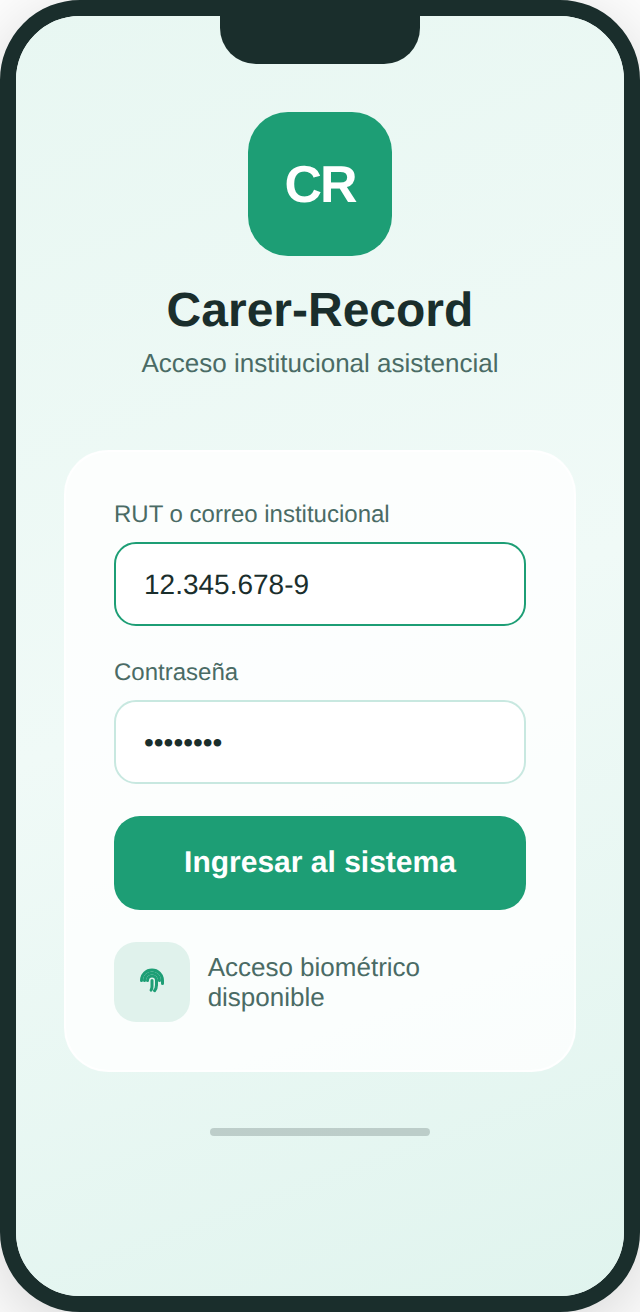
\includegraphics[width=0.2\textwidth]{Imagenes/vista1_autenticacion.png}
    \caption{Vista 1: Autenticación y acceso}
    \label{fig:vista1_autenticacion}
\end{figure}

\subsubsection*{Vista 2: Perfil del paciente activo y línea de tiempo} ~

La Figura~\ref{fig:vista2_timeline} presenta la vista central del sistema y la más crítica para el cambio de turno. Muestra el identificador simbólico del paciente activo, la información mínima del caso y la bitácora cronológica de eventos validados. Cada evento se presenta con su marca temporal, categoría y descripción, permitiendo al médico entrante leer el contexto completo del caso mediante desplazamiento vertical.

\begin{figure}[H]
    \centering
    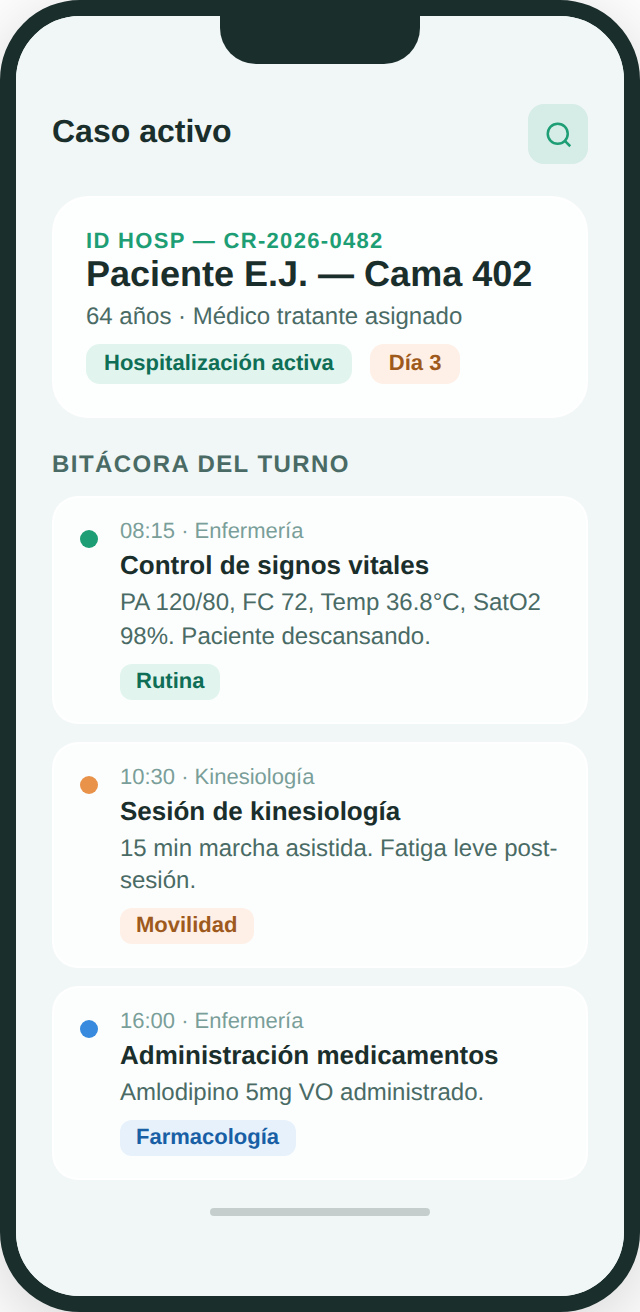
\includegraphics[width=0.2\textwidth]{Imagenes/vista2_linea_de_tiempo.png}
    \caption{Vista 2: Perfil del paciente activo y línea de tiempo}
    \label{fig:vista2_timeline}
\end{figure}

\subsubsection*{Vista 3: Captura de evento por audio o texto} ~

La Figura~\ref{fig:vista3_captura} presenta la vista para registrar un nuevo evento. Ofrece dos opciones de entrada claramente diferenciadas: grabación de audio mediante un botón de gran área táctil y un campo de texto para digitación directa. Las sugerencias de categoría que aparecen en la maqueta histórica no forman parte de los requisitos V4.

\begin{figure}[H]
    \centering
    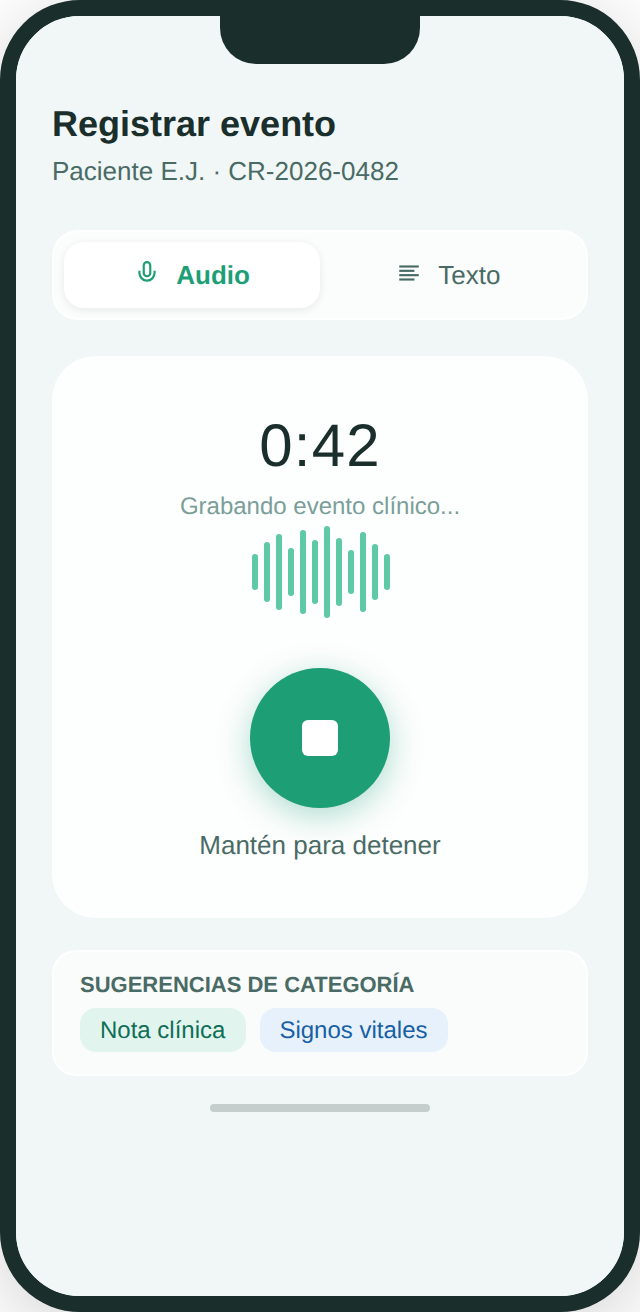
\includegraphics[width=0.2\textwidth]{Imagenes/vista3_captura_evento.png}
    \caption{Vista 3: Captura de evento por audio o texto}
    \label{fig:vista3_captura}
\end{figure}

\subsubsection*{Vista 4: Validación Human-in-the-Loop} ~

La validación con intervención humana (Human-in-the-Loop, HITL) mantiene a la persona autora en control de la revisión del contenido asistido.

La Figura~\ref{fig:vista4_validacion} es una maqueta histórica de revisión. Su transcripción y campos editables ilustran la revisión de contenido; las categorías y el porcentaje de confianza visibles son elementos gráficos históricos, no capacidades requeridas ni mediciones del sistema.

\begin{figure}[H]
    \centering
    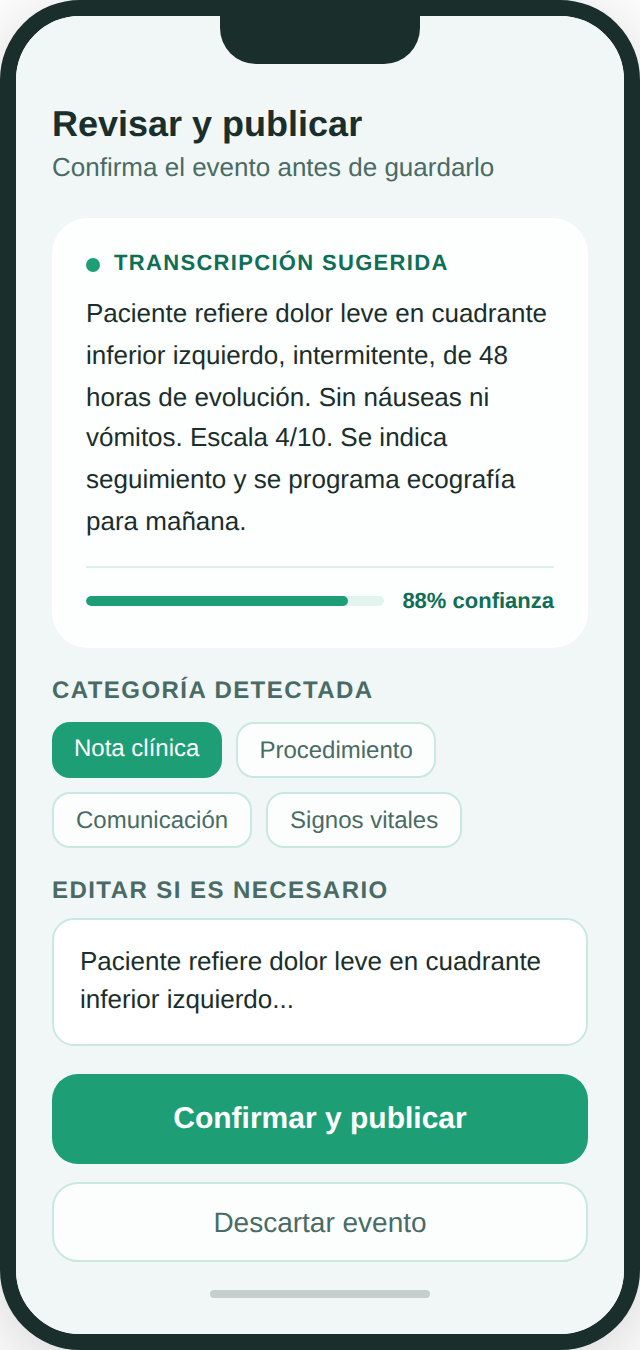
\includegraphics[width=0.2\textwidth]{Imagenes/vista4_validacion.png}
    \caption{Vista 4: Validación Human-in-the-Loop}
    \label{fig:vista4_validacion}
\end{figure}

\subsubsection*{Vista 5: Resumen de período para revisión} ~

La Figura~\ref{fig:vista5_borrador} es una maqueta histórica de resumen. Para el diseño V4, la vista representa la consulta y revisión de un resumen de eventos y notas de un período seleccionado; no supone publicarlo, copiarlo a la FCE ni cerrar un turno. La imagen histórica muestra un control de cierre de turno, que queda fuera del alcance V4 y no representa una función comprometida.

\begin{figure}[H]
    \centering
    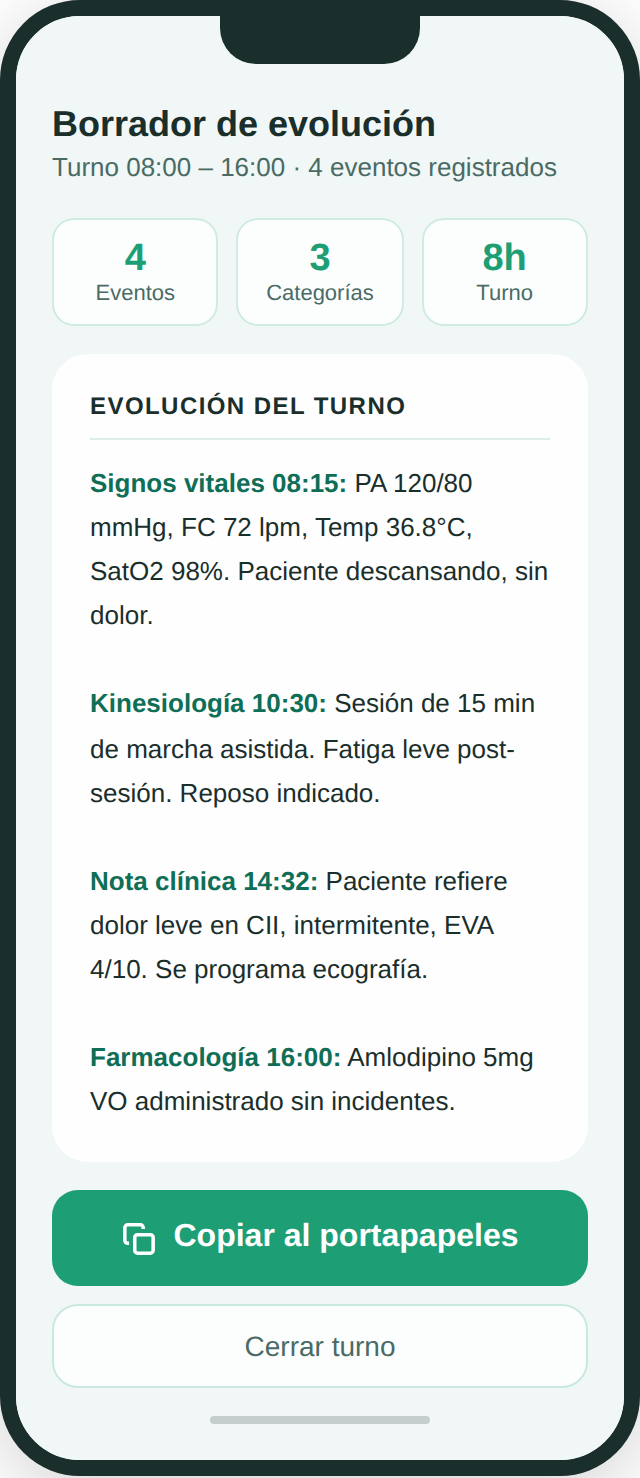
\includegraphics[width=0.2\textwidth]{Imagenes/vista5_borrador_evolucion.png}
    \caption{Vista 5: Resumen de período para revisión (maqueta histórica)}
    \label{fig:vista5_borrador}
\end{figure}

  Las maquetas descritas sirven como referencia visual para los recorridos de usabilidad; sus controles históricos no amplían el alcance funcional V4.
